
\section{Iterative development}
-------------------- re-read all of this ---------------
  The iterative development process has been very useful. It has enabled me to use a few iterations to get to know the problem before trying to create the final solution. If I had started trying to solve the problem completely straight away I would have ended up with a very hap hazard solution.

  Figure~\ref{fig:iteration_loc_history} shows how the three iterations grew over time. The first iteration reached a moderate code size quickly because it solved a small but concrete proof-of-concept problem: generate notes, render them in LilyPond, and optionally generate several independent voices. The second iteration started from a much smaller base and stayed smaller overall because it focused on improving the internal representation and introducing motif-based generation rather than adding many new subsystems. The third iteration grows much more rapidly because it combines a richer data model, explicit constraint handling, harmony support, form planning, rendering workflows, and later SATB-compatible extensions.

  \begin{figure}[h]
    \centering
      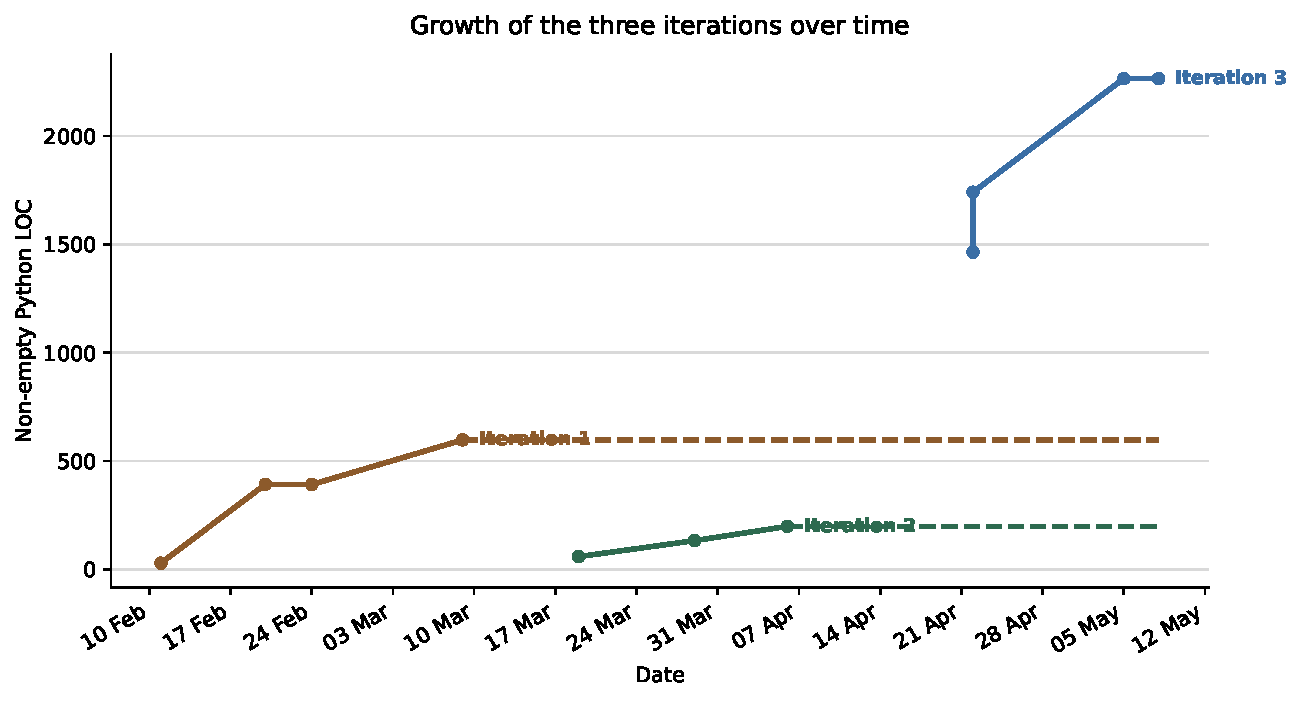
\includegraphics[width=0.95\textwidth]{Figures/05iterations/iteration_loc_history.pdf}
    \caption{Growth of the three iterations over time measured as non-empty Python source lines in the iteration-specific code. Dashed segments indicate that an iteration had been frozen while the thesis work continued.}\label{fig:iteration_loc_history}
  \end{figure}

  This development pattern is important because it shows that the final system did not appear fully formed. Instead, each iteration solved a narrower version of the problem and exposed the next set of weaknesses. The first iteration showed that note generation and rendering were feasible, the second showed that musical reuse required better abstractions, and the third was where the musical rules and architectural structure were finally formalized in a way that could support a larger system.

  \begin{table}[h]
    \centering
    \small
    \begin{tabular}{p{0.34\textwidth}ccc}
      \toprule
      Feature & Iteration 1 & Iteration 2 & Iteration 3 \\
      \midrule
      LilyPond export and audio rendering & yes & yes & yes \\
      Independent multi-voice output & yes & no & yes \\
      Explicit motif reuse & no & yes & yes \\
      Phrase or form planning & no & limited & yes \\
      Automatic tonal harmony plan & no & no & yes \\
      Roman-numeral harmony input & no & no & yes \\
      Melodic soft constraints & no & limited & yes \\
      Rest handling in melody generation & no & no & yes \\
      Register-aware voice profiles and clefs & no & no & yes \\
      SATB-compatible harmonization path & no & no & yes \\
      Descriptive CLI and reproducible seed workflow & limited & limited & yes \\
      \bottomrule
    \end{tabular}
    \caption{Comparison of the main musical and technical capabilities across the three iterations.}\label{tab:iteration_feature_matrix}
  \end{table}

  Table~\ref{tab:iteration_feature_matrix} summarizes the practical differences between the iterations. The main observation is that the first two iterations each solved only part of the problem. Iteration one had rendering and even rudimentary multi-voice support, but the generated melodies were musically weak. Iteration two improved motivic handling and made the code structure easier to reason about, but it still lacked explicit theory-aware constraints. Only the third iteration combines musical structure, reusable abstractions, harmony handling, and a workflow that is robust enough to support the thesis examples.

\section{\ac{AI} development}
  After the first few iterations I had build up a better understanding of not only the problem, but also how I should go about solving it. Having this in the back of my mind when prompt engineering for the \ac{AI} to help me solve it make the end result a lot better than if I tried to solve it using \ac{AI} from the very beginning. 

\section{The system structure}

  The architectural progression is also visible when comparing the system diagrams from the three iteration chapters. Figures~\ref{fig:iter1_architecture}, \ref{fig:iter2_architecture}, and \ref{fig:iter3_architecture} show a clear movement from script-driven generation toward a more modular and theory-aware design.

  \begin{table}[h]
    \centering
    \small
    \begin{tabular}{p{0.24\textwidth}p{0.21\textwidth}p{0.21\textwidth}p{0.21\textwidth}}
      \toprule
      Aspect & Iteration 1 & Iteration 2 & Iteration 3 \\
      \midrule
      Main representation & note and melody objects with limited metadata & motif, bar, and phrase objects & settings, motif, form, harmony, melody, and chorale-related objects \\
      Generation strategy & random local note motion with separate rhythm generation & motif-first phrase generation with small-step filling & weighted search with explicit candidate scoring and harmonic context \\
      Harmony handling & none & none & manual Roman numerals or automatically generated tonal plan \\
      Module structure & small script plus helper modules & clearer separation, but still tightly coupled & dedicated theory, structure, constraints, generator, rendering, and CLI layers \\
      Extensibility & difficult to extend without rewriting & better than iteration 1, but still narrow & designed to support variants, rendering modes, and future multi-voice work \\
      \bottomrule
    \end{tabular}
    \caption{Architectural comparison of the three iterations.}\label{tab:iteration_architecture_comparison}
  \end{table}

  Table~\ref{tab:iteration_architecture_comparison} complements the architecture figures by showing what changed conceptually between the iterations. The most important difference is not just that the third iteration has more modules, but that it has more explicit musical objects and clearer boundaries between responsibilities. This makes it possible to reason about melodic constraints, harmony, rendering, and future extensions separately rather than treating the generator as one monolithic script.

\section{Modules? Different module discussions.}

\section{The generated music}

\section{Future work}
